%!TEX root=kdd15_workshop_main.tex
\section{Evaluation}
\todo{We measure (1) the quality of \ourmethod and (2) the scalability of our implementation.}\\
We ran our distributed experiments on \todo{machine stats here}.

We measured the overall quality of partitions by the \textit{fraction of cut edges} $\lambda$.
\begin{align}\lambda = \frac{\text{Number of edges cut by partition}}{\text{Total number of edges}}\end{align}
The fraction of edges cut demonstrates the quality of the edge minimization aspect of partitioning the graph.

As a baseline, we can compare this to the expected quality of a random $k-$partition.
To estimate this we assume that each block has the same density of nonzeros, so we compute the fraction of nonzeros expected to be in non-diagonal blocks:
\begin{align}\lambda_r = \frac{k^2 - k}{k^2} = \frac{k-1}{k} \end{align}

Any partitioner that produces a partition with $\lambda < \lambda_r$ has thus improved the parallel locality of the graph ordering, so we present $\lambda_{r,k}$ along with our results.

\subsubsection{SNAP Data Set}
\todo{We need to select a subset of these graphs to show, otherwise the plots are utterly impossible to read.}\\
The SNAP data set is a set of real-world networks collected by Jure Leskovec and collaborators~\cite{Leskovec-data}. Many networks in the collection are power-law and scale-free representatives of social networks (such as collaboration networks, citation networks, email networks, and web graphs). We consider these to be ideal targets for streaming partitioning, because these domains are producing the vast majority of the `big-data' that is difficult to partition using traditional methods.

We also speculate (but have no proof) that the `random' structure of scale-free networks better suits the random quality of streaming graph partitioning, whereas a spatially-oriented graph would be poorly suited (for instance, in a grid, a streaming partitioner would create many local pockets for one particular partition, whereas a spatial partitioner would recognize that the graph could be geometrically bisected).

In Figure~\ref{table:big} we show the main properties of graphs in the SNAP database, as well as the performance of our streaming partitioner on them, for $k=2$ and $k=8$.

\begin{figure*}
\caption{Basic properties of graphs in SNAP data set~\cite{Leskovec-data}, and $\lambda$ for one pass. $\lambda_{r,2}=0.5,\lambda_{r,8}=0.87$}
\rowcolors{2}{blue!05}{blue!15}
\centering
{ \begin{tabular}{ *7l }    \toprule
\label{table:big}
\emph{Data Set} & $N$ & $nnz$ & \emph{sym} & \emph{power-law?} & $\lambda, k=2$ & $\lambda, k=8$ \\\midrule
% amazon0302 & 262111 & 1234877 & no & yes & 0.202&0.37\\
% amazon0312 & 400727 & 3200440 & no & yes & 0.212&0.38\\
% amazon0505 & 410236 & 3356824 & no & yes & 0.206&0.37\\
amazon0601 & 403394 & 3387388 & no & yes & 0.203&0.36\\
% as-735 & 7716 & 26467 & yes & yes & 0.207&0.44\\
as-Skitter & 1696415 & 22190596 & yes & yes & 0.166&0.324\\
ca-AstroPh & 18772 & 396160 & yes & yes & 0.232&0.413\\
% ca-CondMat & 23133 & 186936 & yes & yes & 0.214&0.398\\
% ca-GrQc & 5242 & 28980 & yes & yes & 0.128&0.241\\
% ca-HepPh & 12008 & 237010 & yes & yes & 0.082&0.192\\
% ca-HepTh & 9877 & 51971 & yes & yes & 0.202&0.378\\
cit-HepPh & 34546 & 421578 & no & yes & 0.343&0.646\\
% cit-HepTh & 27770 & 352807 & no & yes & 0.360&0.605\\
cit-Patents & 3774768 & 16518948 & no & yes & 0.402&0.726\\
% email-Enron & 36692 & 367662 & yes & yes & 0.132&0.407\\
email-EuAll & 265214 & 420045 & no & yes & 0.280&0.538\\
% Oregon-1 & 11492 & 46818 & yes & yes & 0.224&0.406\\
% Oregon-2 & 11806 & 65460 & no & yes & 0.185&0.429\\
p2p-Gnutella04 & 10879 & 39994 & no & yes & 0.415&0.747\\
% roadNet-CA & 1971281 & 5533214 & yes & no & 0.186&0.36\\
% roadNet-PA & 1090920 & 3083796 & yes & no & 0.188&0.36\\
roadNet-TX & 1393383 & 3843320 & yes & no & 0.185&0.358\\
% soc-Epinions1 & 75888 & 508837 & no & yes & 0.173&0.34\\
soc-LiveJournal1 & 4847571 & 68993773 & no & yes &0.234& 0.463\\
% soc-sign-epinions & 131828 & 841372 & no & yes &0.173&0.34\\
% soc-Slashdot0811 & 77360 & 905468 & no & yes &0.179&0.417\\
soc-Slashdot0902 & 82168 & 948464 & no & yes &0.236&0.382\\
% web-BerkStan & 685230 & 7600595 & no & yes &0.187&0.301\\
web-Google & 916428 & 5105039 & no & yes &0.189&0.336\\
% web-NotreDame & 325729 & 1497134 & no & yes &0.204&0.345\\
% web-Stanford & 281903 & 2312497 & no & yes &0.154&0.34\\
wiki-Talk & 2394385 & 5021410 & no & yes &0.411&0.752\\
% wiki-Vote  & 8297 & 103689 & no & yes &0.409&0.688\\
 \hline
\end{tabular}\par
}
\end{figure*}

As a note, the ratio of change in $\lambda$ from $k=2$ to $k=8$ was for the vast majority of cases within 1.5 and 2.2. This shows a decent deal of scalability.

We also note Figure~\ref{fig:4}, which illustrates the result of the streaming algorithm on a more spacial network (roadNet-CA). The `local' nonzeros are those points in the 8 diagonal blocks, while the `remote' edges are those outside. While a good partitioner would concentrate the vast majority of elements along the diagonal (which is possible because the graph has very high diameter), the streaming partitioner fails to recognize this quality, and each partition has vertices distributed somewhat randomly through the network. Nonetheless, the partition is decent (only 18 percent of edges are cut).

\begin{figure}[h!]
\centering
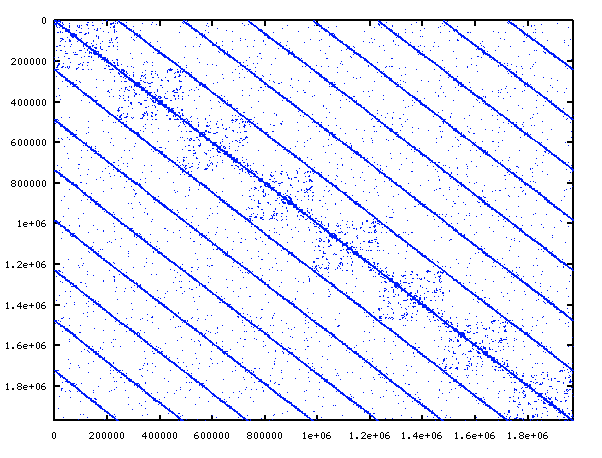
\includegraphics[width=0.8\columnwidth] {figures/roadNet-CA8.png}
\caption[Caption for]{Spy plot of roadNet-CA 8-partition ($\lambda=0.177$). This illustrates how a streaming algorithm cannot take into account the spatial/planar properties of a graph.}
\label{fig:4}
\end{figure}

\subsubsection{Synthetic Graphs}
To generate synthetic graphs we used the Stanford Network Analysis Platform (SNAP) random graph generator.

\begin{figure}[h!]
\centering
  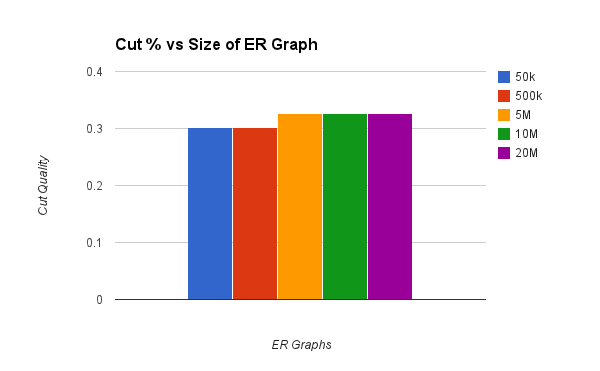
\includegraphics[width=0.8\columnwidth]{figures/lambda_ER.png}
  \caption{Partition quality of ER graphs with same $p$-value}
  \label{fig:lambdaer}
\end{figure}

\begin{figure}[h!]
\centering
  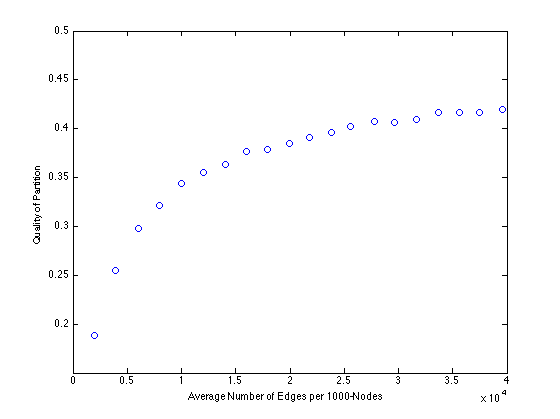
\includegraphics[width=0.8\columnwidth]{figures/varied_er_p.png}
  \caption{Partition quality of an ER graph with varying $p$-value, $k=2$}
  \label{fig:lambdap}
\end{figure}



In Figure~\ref{fig:lambdaer} we investigated the streaming graph partitioner on Erdos-Renyi graphs with a widely varying number of nodes, but the same probability $p$. From our small sample set, there appears to be little change in partition quality.

In Figure~\ref{fig:lambdap} however, we increase the $p$-value on a single ER graph. We see that the partition quality significantly decreases. This is to be expected of all partitioners in general. In fact, for E-R graphs, the critical $p$-value for which the optimal edge cut is equal to the expected average random partition is relatively simple to identify~\cite{journals/cj/GanleyH94}

\section{Additional Passes}
Another operation we explored was performing additional passes of partitioning on a pre-partitioned graph. The reasoning is that the partitioner is fast enough that it may be faster to do $n$ passes than use a slower mainstream graph partitioner, for some value of $n$. To explore this idea, we perform a number of passes on the SNAP data set, and observe qualitatively which graphs benefit the most.

The algorithm is simple: once we have computed the first partition, we retain the original partition mapping. Then, as we make another pass, we compute the new objective function using the partition mapping that has already been filled in. Vertices may then be switched to new partitions. This mitigates poor partitioning decisions that may have been made at the beginning of the algorithm, when there was not as much information.

Figures~\ref{fig:01},\ref{fig:02},\ref{fig:03},\ref{fig:04} show the improvement of $\lambda$ as we continue to make passes over selected networks. Significant improvements are made for the vast majority of data sets.

We hope to contrast this performance to that of METIS in the future. (We have implemented a METIS partitioner for comparison but it currently encounters a segmentation faults with some frequency).



\begin{figure}[h!]
\centering
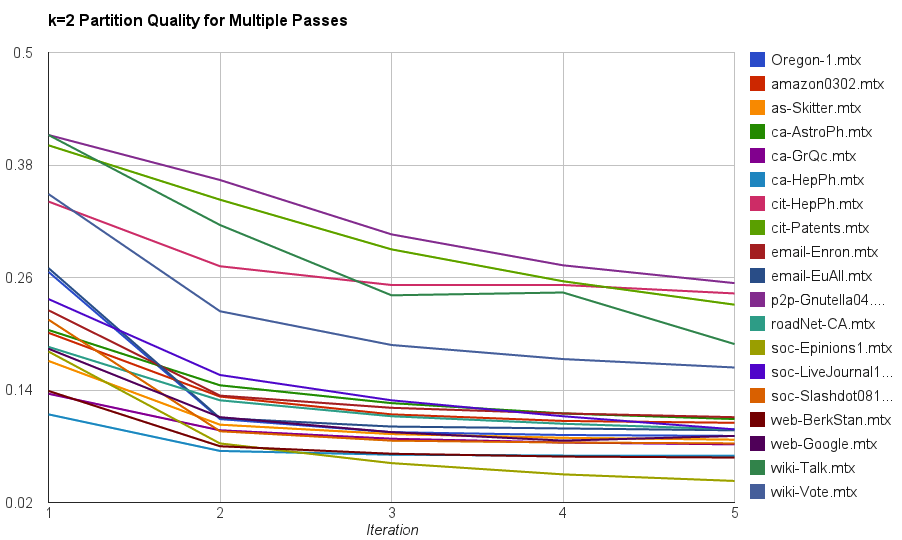
\includegraphics[width=0.8\columnwidth] {figures/2partlambda}
\caption[Caption for]{Improvement in $\lambda$ over 5 WDG passes, $k=2$.}
\label{fig:01}
\end{figure}

\begin{figure}[h!]
\centering
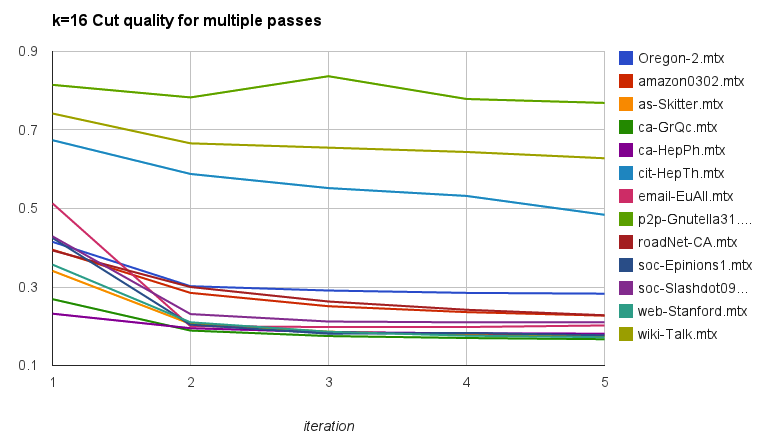
\includegraphics[width=0.8\columnwidth] {figures/16partlambda}
\caption[Caption for]{Improvement in $\lambda$ over 5 WDG passes, $k=16$.}
\label{fig:02}
\end{figure}

\begin{figure}[h!]
\centering
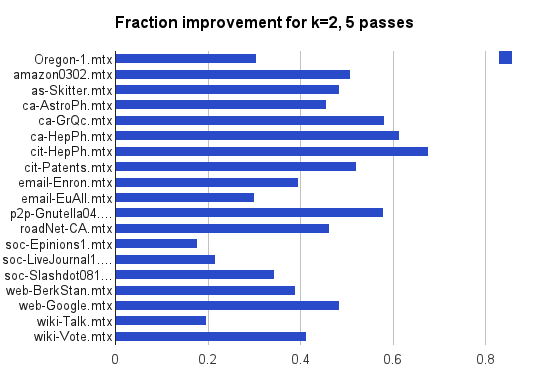
\includegraphics[width=0.8\columnwidth] {figures/2partfrac}
\caption[Caption for]{Fraction Improvement in $\lambda$ after 5 WDG passes, $k=2$.}
\label{fig:03}
\end{figure}

\begin{figure}[h!]
\centering
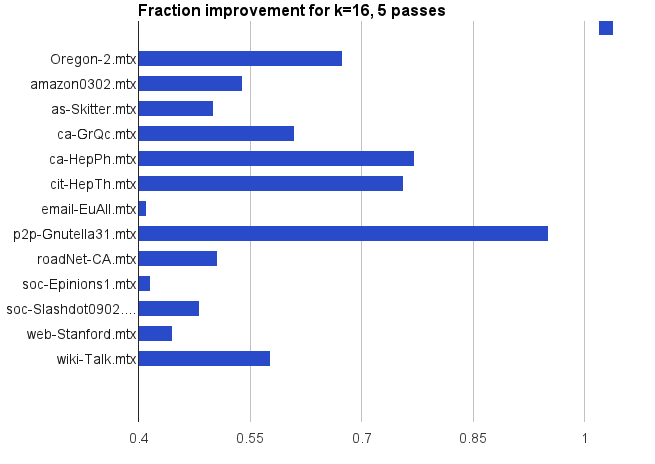
\includegraphics[width=0.8\columnwidth] {figures/16partfrac}
\caption[Caption for]{Fraction Improvement in $\lambda$ after 5 WDG passes, $k=16$.}
\label{fig:04}
\end{figure}

\begin{figure}[h!]
\centering
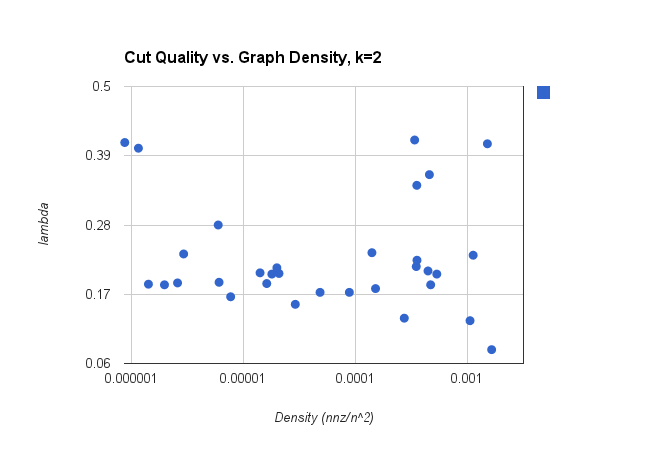
\includegraphics[width=0.8\columnwidth] {figures/cutvsdens}
\caption[Caption for]{Cut quality vs nonzero density for each of the graphs in Figure~\ref{table:big}. The graph shows no noticeable correlation.}
\end{figure}


\section{Analysis}

One set of outlying (poorly-performing) data points we noticed was the Gnutella networks.
While Gnutella networks exhibit power-law-like topology, elements of their algorithm truncate nodes from ever becoming extremely large. This does not match other social network topologies.
The data sets also have extremely low clustering coefficient and a very small number of closed triangles. \cite{Ripeanu:2002:MGN:613352.613670}. This makes the Gnutella data set an anomaly compared to the others.

Other data from real-world was harder to analyze -- there are not enough wide differences between data sets' results to draw strong conclusions.
However, the encouraging side to this is that every partition was unexpectedly good.
While Power-Law graphs are overwhelmingly considered to be difficult to partition~\cite{Abou-Rjeili:2006:MAP:1898953.1899055}, we have demonstrated that a very simple, fast, one-pass algorithm is capable of significantly reducing communication in their parallel computation, and that several further passes can further reduce edge cut by up to a factor of 3. Isolated comparisons we have made to the state-of-the-art partitioner METIS show that these results are competitive (usually within a factor of 2).
This makes streaming partitioning a valid alternative to be integrated within distributed-memory, on-the-fly algorithms for big-data.

One interesting fact of note is that when we ran multiple passes on the graphs, one partition would become populated by very high-degree vertices.
We see this in Figure~\ref{fig:dense}. We attribute this to the notion that scale-free graphs have a ``dense core'' surrounded by a less-dense periphery.
This is qualitatively noticed when scale-free graphs are embedded in a spectral space~\cite{Lang04findinggood}.
This dense partition tends to strongly emerge as we continue to make further passes of the streaming algorithm, and is what we attribute to the improvement in overall partition quality.

\begin{figure}[h!]
\centering
  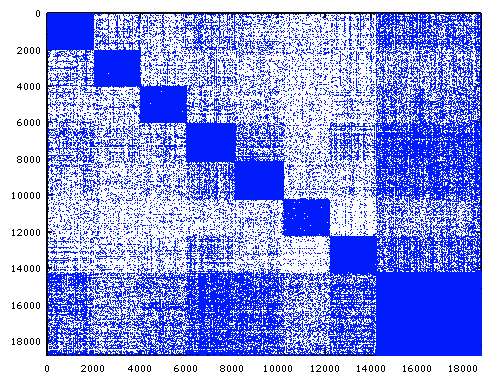
\includegraphics[width=0.8\columnwidth]{figures/astroPh8.png}
  \caption{Spy plot of ca-AstroPh 8-partition ($\lambda=0.253$). Note the denser, high-degree subgraph.}
  \label{fig:dense}
\end{figure}


